\section{Background}
\subsection{Word Embeddings}
A word embedding is a function mapping from words to their continuous vector representations.
The purpose of this method is to encode relevant syntactic and semantic features of words as relationships among their representation vectors.
Usually, word embeddings are trained on large, unlabeled corpus~\cite{glove,word2vec} and then fine-tuned with respect to specific NLP tasks~\cite{treeLSTM,KimCNN}.   
Pre-learned word presentations have been applied widely and become the ``secret sauce'' for the success of recent NLP systems~\cite{Luong_betterword}.
\paragraph{Matrix presentation of sequences of words}
Given any sentence \(s\) of length \(n\), we denote \(x_i \in \mathbb{R}^d\) as a vector presentation of word-\(i\)th in the sentence.
The first word in a sentence is word-\(0\)th.
In case the sentence is padded with dummy words on its left, these padded dummy words are indexed by negative integers.
Any sequence of words in the sentence which start at word-\(i\)th and end at word-\(j\)th can be presented as the following matrix:
\begin{align}
X_{i:j} &= x_i \oplus x_{i+1} \oplus ... \oplus x_{j} &\label{concat}
\end{align}
In Eq.\eqref{concat}, \(\oplus\) is concatenation operator which result in the matrix \(X_{i:j} \in \mathbb{R}^{d \times (j-i+1)}\).
\subsection{Convolution and Pooling}
Convolution Neural Networks (CNNs) have been proven to be effective models for the task of sentence-level sentiment analysis~\cite{KimCNN, DCNN,2-layer-cnn}.
Convolution Neural Networks usually constructed by staking up multiple convolution, pooling and fully connected layers.
\subsubsection{Convolution Layer}
Given that \(F\) is the set of all filters of the convolution layer, for any filter \(v \in F\) which has window size \(l\) and set of parameters \(\theta^{(v)} = \{ W^{(v)}, b^{(v)} | W^{(v)} \in \mathbb{R}^{d \times l}, b^{(v)} \in \mathbb{R}\}\), filter \({v}\) is applied on any sequence of word-\(i\)th to word-\((i+l-1)\)th through the following equation:
\begin{align}
c^{(v)}_j &= f(W^{(v)} \otimes X_{i:i+l-1} + b^{(v)}) &\label{filter}
\end{align}
In Eq.\eqref{filter}, operator \(\otimes\) is the Hadamard product~\cite{element-prod}.  
\(b \in \mathbb{R}\) as bias term and \(f\) is an activation function.
For indexing, \(j = i + x\) with \(x \in \mathbb{N}\) and \(0 \leq x < l\).
If half-padding policy is employed then \(j = i + \floor{\frac{l}{2}}\).

By slicing the filter \(v\) through the sentence (i.e. applying the filter \(v\) on different sequences of length \(l\) along the sentence) we can get vector \(c^{(v)} = [c^{(v)}_0, c^{(v)}_1~\cdots]\) which is a feature map of the sentence~\(s\).
The length of the feature map \(c^{(v)}\) depends on the length of the input sentence.
Additionally, the length of \(c^{(v)}\) also depends on the way filter \(v\) was slided through the sentence and its window size \(l\)~\cite{conv-arith}.
In summary, each filter produces a variable-length feature map of the sentence.
As a result, when applying a convolution layer on a sentence, we get a set of variable-length feature maps.
\subsubsection{Max Pooling Layer}
For dealing with the problem of variable-length feature maps, several types of max pooling layer was employed.
In general, given a input vector \(i\), a \(k\)-max pooling layer reduces the size of vector \(i\) by extracting the largest \(k\) entries from \(i\).
In case \(k = 1\) the pooling layer is called max-over-time pooling~\cite{nlp-scratch,KimCNN}.
Apart from being treated as a hyper-parameter, \(k\) can also be parameterized with respect to the length of the input sentence, in which case, the pooling layer is called dynamic k-max pooling~\cite{DCNN}.
\subsection{Recurrent Neural Network}
By definition, Recurrent Neural Networks are any Neural Networks which have at least a recurrent connection~\cite{rnn-def}.
\subsubsection{Long Short Term Memory unit}\label{sec:lstm}
Given a input sequence \(I = (i_0,\ldots,i_n), \forall t, i_t \in \mathbb{R}^n\), Long Short Term Memory unit can be expressed as the following recursive formula~\cite{treeLSTM}:
\begin{align}
w_t &= \sigma(W^{(w)}i_t + U^{(w)}h_{t-1} + b^{(w)}) \label{eq:lstm-input-gate}&\\
f_t &= \sigma(W^{(f)}i_t + U^{(f)}h_{t-1} + b^{(f)}) \label{eq:lstm-forget-gate}&\\
o_t &= \sigma(W^{(o)}i_t + U^{(o)}h_{t-1} + b^{(o)}) \label{eq:lstm-output-gate}&\\
u_t &= tanh(W^{(u)}i_t + U^{(u)}h_{t-1} + b^{(u)}) \label{eq:lstm-update-gate}&\\
c_t &= r_t \otimes u_t + f_t \otimes c_{t-1} \label{eq:longterm-mem}&\\
h_t &= o_t \otimes tanh(c_t) \label{eq:temperal-mem}&
\end{align}
In the formula above, operator \(\otimes\) is the Hadamard product~\cite{element-prod}.
The role of \(h_t\) in LSTM unit is similar to its role in Vanilla Recurrent unit.
Traditionally, \(w_t\), \(f_t\) and \(o_t\) are called input/write gate, forget/deallocate gate and output/read gate respectively.
In addition, \(c_t\) is called memory cell.

Consistently, LSTM outperform Vanilla RNN in most tasks.
Intuitively, LSTM mitigates the problem of vanishing gradient by updating their memory through adding~\cite{evaluate-GRU}, although gradients still decrease through time, it is not exponentially~\cite{Graves-thesis}.
\subsection{Recursive Neural Network}
In most cases, to understand a sentence, we have to understand the phrases composing it.
Analogously, to understand a phrase, we have to understand the phrases and words composing it.
Recursive Neural Networks were mainly inspired by this idea~\cite{treeLSTM}.
Given a sentence and its parse tree, a Recursive Neural Network composes the vector presentation of the sentence by applying it composition function at each node of the parse tree in a bottom-up manner.
For demonstration, parse tree of the phrase ``is very interesting'' and its composing process using a Recursive Neural Network are illustrated in Fig.\ref{fig:example-parse} and Fig.\ref{fig:example-compose} respectively~\cite{tag-embedding-rnn}.


\begin{figure}% [H] meow note: H cause weird bug
	\centering
	% 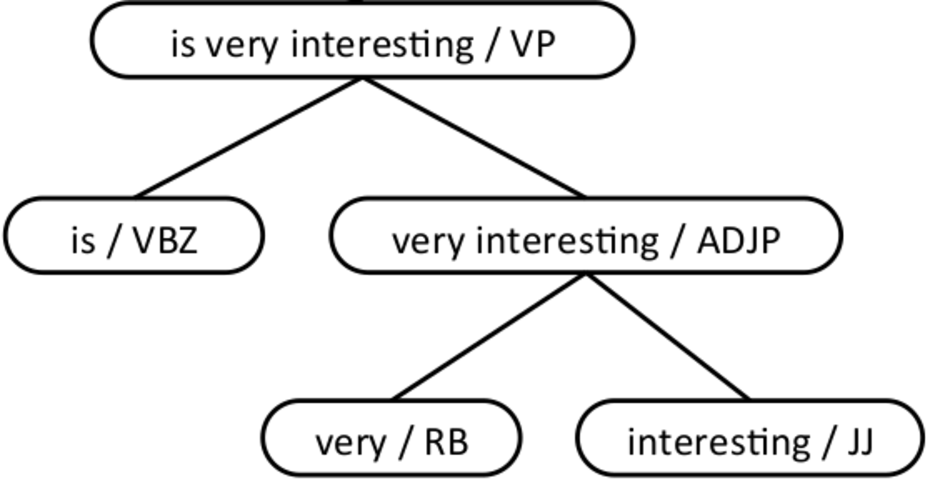
\includegraphics[scale=0.4]{figure/example-parse}
	%\resizebox{.4\textwidth}{!}{%
		\begin{tikzpicture}
		\node [sq] (v1) at (1,-1) {root};
		\node [sq] (v2) at (1,-2) {S};
		\node [sq] (v3) at (-1.5,-3) {NP};
		\node [sq] (v6) at (-1.5,-4) {PRP};
		\node [cir] (v7) at (-1.5,-5.5) {I};
		\node [sq] (v4) at (1,-3) {VP};
		\node [sq] (v8) at (0,-4) {VBP};
		\node [cir] (v10) at (0,-5.5) {feed};
		\node [cir] (v11) at (1.5,-5.5) {the};
		\node [cir] (v12) at (3,-5.5) {cat};
		\node [cir] (v13) at (4.5,-5.5) {.};
		\node [sq] (v9) at (2,-4) {NP};
		\node [sq] (v5) at (4.5,-3) {.};
		\draw [->] (v1) edge (v2);
		\draw [->] (v2) edge (v3);
		\draw [->] (v2) edge (v4);
		\draw [->] (v2) edge (v5);
		\draw [->] (v3) edge (v6);
		\draw [->] (v6) edge (v7);
		\draw [->] (v4) edge (v8);
		\draw [->] (v4) edge (v9);
		\draw [->] (v8) edge (v10);
		\draw [->] (v9) edge (v11);
		\draw [->] (v9) edge (v12);
		\draw [->] (v5) edge (v13);
		\end{tikzpicture}
	%}
	\caption[Constituency parse tree for the phrase ``is very interesting'']{Constituency parse tree for the phrase ``is very interesting''.}
	\label{fig:example-parse}
\end{figure}

\begin{figure} % [H] meow note: H cause weird bug
	\centering
	% 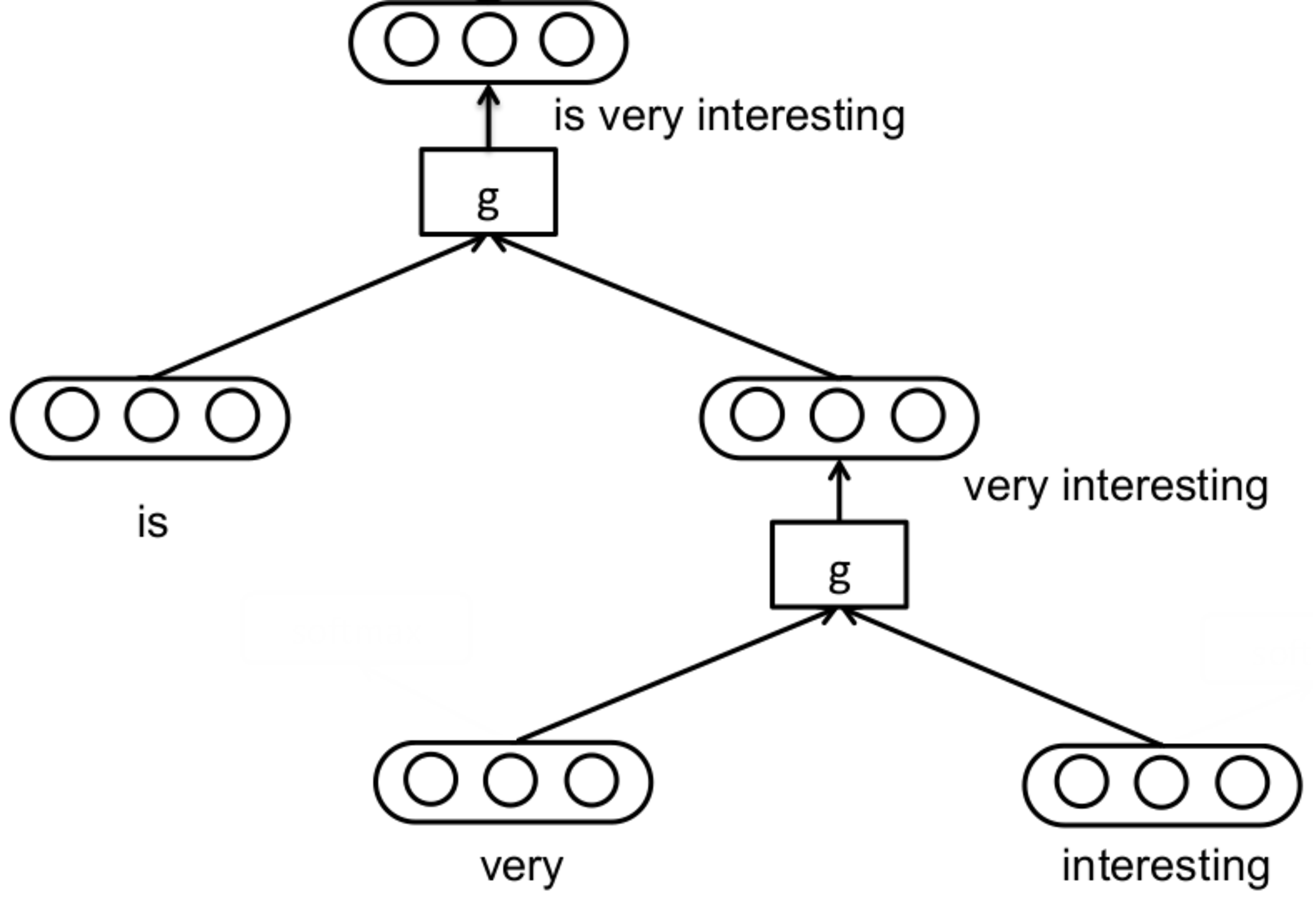
\includegraphics[scale=0.3]{figure/example-compose}
	
\begin{tikzpicture}
\node [sqvec] (v1) at (3,0) {
	\node[cirsmall] {}; &\node[cirsmall] {}; &\node[cirsmall] {}; \\
};      
\node [sqvec] (v3) at (5,0) {
	\node[cirsmall] {}; &\node[cirsmall] {}; &\node[cirsmall] {}; \\
};      
\node [sqvec] (v4) at (4,2) {
	\node[cirsmall] {}; &\node[cirsmall] {}; &\node[cirsmall] {}; \\
};      
\node [sqvec] (v6) at (1,2) {
	\node[cirsmall] {}; &\node[cirsmall] {}; &\node[cirsmall] {}; \\
};      
\node [sqvec] (v8) at (-0.5,4) {
	\node[cirsmall] {}; &\node[cirsmall] {}; &\node[cirsmall] {}; \\
};      
\node [sqvec] (v7) at (2.5,4) {
	\node[cirsmall] {}; &\node[cirsmall] {}; &\node[cirsmall] {}; \\
};      
\node [sqvec] (v10) at (1,6) {
	\node[cirsmall] {}; &\node[cirsmall] {}; &\node[cirsmall] {}; \\
};      
\node [sq] (v2) at (4,1) {g};
\node [sq] (v5) at (2.5,3) {g};
\node [sq] (v9) at (1,5) {g};

\node at (-0.5,3.5) {I};
\node at (1,1.5) {feed};
\node at (3,-0.5) {the};
\node at (5,-0.5) {cat};
\node at (5,1.5) {the cat};
\node at (4,3.5) {feed the cat};
\node at (2.5,5.5) {I feed the cat};

\draw [arrow] (v1) edge (v2);
\draw [arrow] (v3) edge (v2);
\draw [arrow] (v2) edge (v4);
\draw [arrow] (v4) edge (v5);
\draw [arrow] (v6) edge (v5);
\draw [arrow] (v5) edge (v7);
\draw [arrow] (v8) edge (v9);
\draw [arrow] (v7) edge (v9);
\draw [arrow] (v9) edge (v10);
\end{tikzpicture}
	\caption[Applying Recursive Neural Network on the phrase ``is very interesting'']{Applying Recursive Neural Network on the Constituency parse tree of the phrase ``is very interesting''.
		The composition function of this network is denoted as \textbf{g}.}
	\label{fig:example-compose}
\end{figure}

\begin{figure} % [H] meow note: H cause weird bug
	\centering
	% 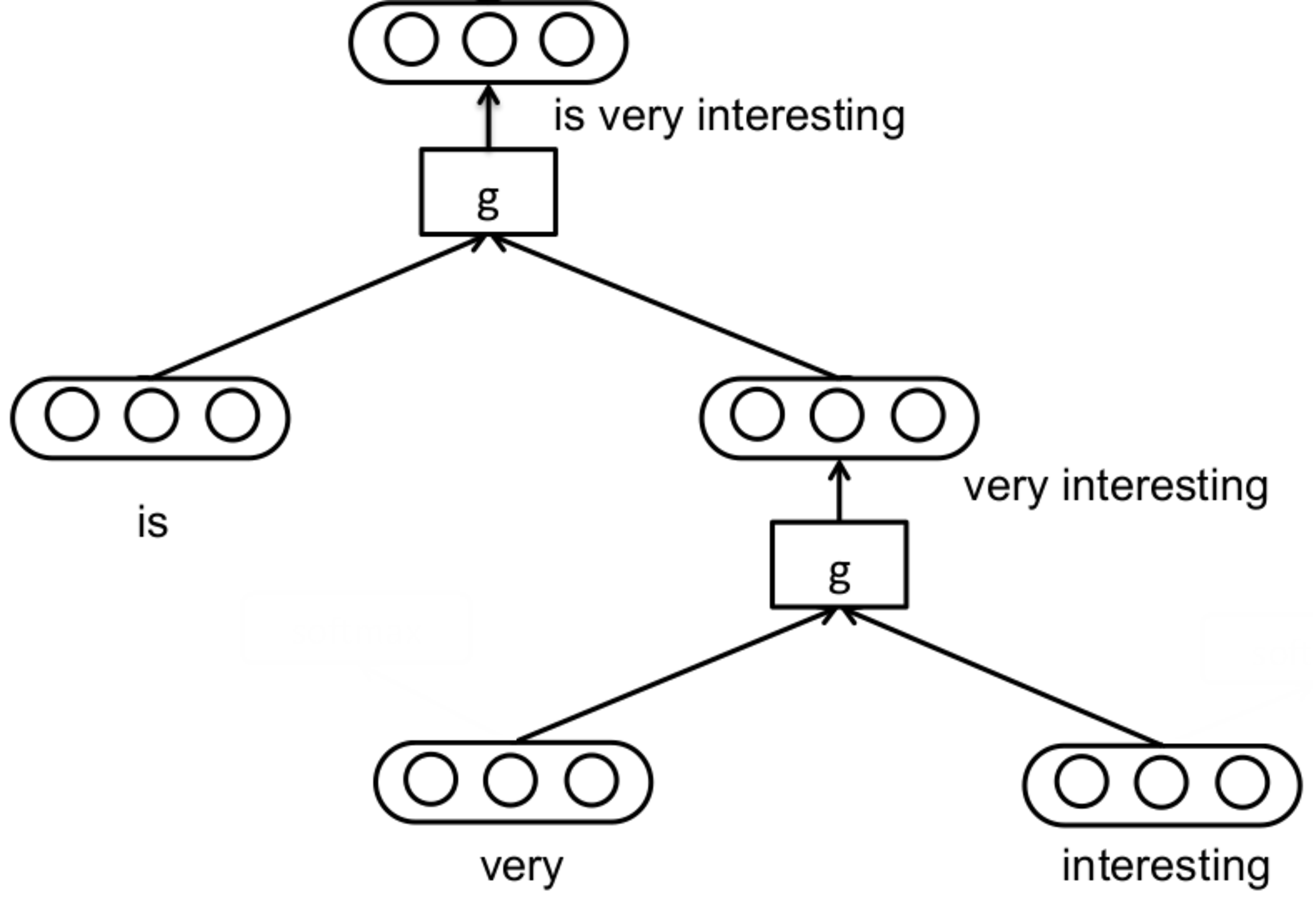
\includegraphics[scale=0.3]{figure/example-compose}
	\usetikzlibrary{matrix}
\usetikzlibrary{patterns}
\tikzset{
	sq1/.style={rectangle, minimum width=0.5cm, minimum height=0.5cm, text centered, draw=black},
	sq1m/.style={rectangle, minimum width=0.7cm, minimum height=0.3cm, text centered, draw=black},
	sq1p/.style={rectangle, minimum width=0.5cm, minimum height=0.5cm, text centered, draw=black, pattern=north west lines},
	circ/.style={circle, minimum width=0.3cm, minimum height=0.3cm, text centered, draw=black},
	arrow/.style={thick,->},
	sqvec/.style={matrix,matrix of nodes,nodes in empty cells},
}
\tikzstyle{cir} = [circle, minimum width=0.7cm, minimum height=0.7cm, text centered, draw=black ]

\begin{tikzpicture}
\node [sqvec,nodes={circ},      
every even row/.style = { nodes={fill=red!60}},
every odd row/.style = { nodes={fill=black!100}}] (c1) at (1.5,8.5) {
	\\
	\\ 
};  

\node [sqvec,nodes={circ},      
every even row/.style = { nodes={fill=red!60}},
every odd row/.style = { nodes={fill=black!100}}] (c2) at (2,8.5) {
	\\
	\\ 
};  

\node [sqvec,nodes={circ},      
every even row/.style = { nodes={fill=red!60}},
every odd row/.style = { nodes={fill=black!100}}] (c3) at (2.5,8.5) {
	\\
	\\ 
};  

\node [sqvec,nodes={circ},      
every even row/.style = { nodes={fill=red!60}},
every odd row/.style = { nodes={fill=black!100}}] (c4) at (3,8.5) {
	\\
	\\ 
};  

\node [sqvec,nodes={circ},      
every even row/.style = { nodes={fill=red!60}},
every odd row/.style = { nodes={fill=black!100}}] (c5) at (3.5,8.5) {
	\\
	\\ 
};  


\node [sqvec,column sep=-\pgflinewidth,nodes={sq1}] (v) at (2.5,5.5) {
	&&&&\\
	&&&&\\
	&&&&\\
};   

\node [sqvec,column sep=-\pgflinewidth,nodes={sq1p}] (v1) at (1,5.5) {
	\\
	\\
	\\
};   
\node [sqvec,column sep=-\pgflinewidth,nodes={sq1p}] (v2) at (0.5,5.5) {
	\\
	\\
	\\
};   
\node [sqvec,column sep=-\pgflinewidth,nodes={sq1p}] (v3) at (4,5.5) {
	\\
	\\
	\\
};   
\node [sqvec,column sep=-\pgflinewidth,nodes={sq1p}] (v4) at (4.5,5.5) {
	\\
	\\
	\\
};   

\draw (v1-1-1.north west) -- (c1-2-1.west); % inner left
\draw (v-1-3.north west) -- (c1-2-1.east); % inner right
\draw (v2-1-1.north west) -- (c1-1-1.west); % outer left
\draw (v-1-4.north west) -- (c1-1-1.east); % outer right

\draw (v-1-1.north west) -- (c2-2-1.west); % inner left
\draw (v-1-4.north west) -- (c2-2-1.east); % inner right
\draw (v1-1-1.north west) -- (c2-1-1.west); % outer left
\draw (v-1-5.north west) -- (c2-1-1.east); % outer right

\draw (v-1-2.north west) -- (c3-2-1.west); % inner left
\draw (v-1-5.north west) -- (c3-2-1.east); % inner right
\draw (v-1-1.north west) -- (c3-1-1.west); % outer left
\draw (v-1-5.north east) -- (c3-1-1.east); % outer right

\draw (v-1-3.north west) -- (c4-2-1.west); % inner left
\draw (v-1-5.north east) -- (c4-2-1.east); % inner right
\draw (v-1-2.north west) -- (c4-1-1.west); % outer left
\draw (v3-1-1.north east) -- (c4-1-1.east); % outer right

\draw (v-1-4.north west) -- (c5-2-1.west); % inner left
\draw (v3-1-1.north east) -- (c5-2-1.east); % inner right
\draw (v-1-3.north west) -- (c5-1-1.west); % outer left
\draw (v4-1-1.north east) -- (c5-1-1.east); % outer right


\node [sq1m] (v8) at (2,10.5) {};
\node [sq1m] (v7) at (1.5,10) {};
\node [sq1m] (v6) at (3,10) {};
\node [sq1m] (v5) at (2.5,9.5) {};
% \draw  (c3) edge (v5);
% \draw  (c4) edge (v5);
\draw  (v5) edge (v6);
% \draw  (c5) edge (v6);
% \draw  (c1) edge (v7);
\draw  (v7) edge (v8);
% \draw  (c2) edge (v7);
\draw  (v6) edge (v8);



\node at (0.5,4.5) {pad};
% \node at (1,4) {pad};
\node at (1.5,4.5) {$x_1$};
\node at (2,4.5) {$x_2$};
\node at (2.5,4.5) {$x_3$};
\node at (3,4.5) {$x_4$};
\node at (3.5,4.5) {$x_5$};
\node at (4.5,4.5) {pad};
% \node at (4.5,4) {pad};

\node at (-1,8.5) {Convolution};
\node at (-1,5.5) {Word vectors};
\node at (-1,10) {Tree-LSTM};

% connect lstm to circle
\draw  (v7) edge (c1-1-1.north);
\draw  (v7) edge (c2-1-1.north);
\draw  (v5) edge (c3-1-1.north);
\draw  (v5) edge (c4-1-1.north);
\draw  (v6) edge (c5-1-1.north);
\end{tikzpicture}
	\caption[mewo write sth here]{meow write sth here}
	\label{fig:cnntreelstm}
\end{figure}

The core idea behind the design of Tree-LSTMs is to generalize the LSTMs for tree-structured inputs.
Tree-LSTMs were able to archive state-of-the-art performance on two tasks: predicting the semantic relatedness of two sentences (SemEval 2014, Task 1~\cite{SemeEvalTask1}) and sentiment classification (Stanford Sentiment Treebank~\cite{socher2013recursive}).

Let \(d\) be the size of the input vectors, \(r
\) be the size of the memory cell and \(z\) be the number of sentiment classes. 

\paragraph{Leaf module}
Given any input vector \(x \in \mathbb{R}^d\), the calculation steps inside the leaf module can be expressed as follow:
\begin{align}
o &= \sigma{\left( W^{(o)} x + a^{\left(o\right)}\right)} & \\
c &= W^{(c)} x + a^{(c)} & \\
h &= o \odot \tanh{\left(c\right)} &
\end{align}

In this module, \(W^{(o)}, W^{(c)} \in \mathbb{R}^{r \times d}\) and \(a^{\left(o\right)}, a^{(c)} \in \mathbb{R}^r\).

\paragraph{Composer module}
Given the input vectors \({h_l}\), \({c_l}\) from the left child node and \({h_r}\), \({c_r}\) from the right child node, the calculation steps inside the composer module can be expressed as follow:
\begin{align}
i &= \sigma{ \left(U_l^{(i)} h_{l} + U_r^{(i)} h_{r} + b^{(i)} \right) } &\\
f_{l} &= \sigma{\left(U_{l}^{(l)} h_{l} + U_{r}^{(l)} h_{r} + b^{(f)}\right)} & \\
f_{r} &= \sigma{\left(U_{l}^{(r)} h_{l} + U_{r}^{(r)} h_{r} + b^{(f)}\right)} & \\
o &= \sigma{\left( U_l^{(o)} h_{l} + U_r^{(o)} h_{r} + b^{(o)}\right)} &\\
u &= \tanh{\left( U_l^{(u)} h_{l} + U_r^{(u)} h_{r} + b^{(u)}\right)} &\\
c &= i \odot u + f_{l} \odot c_{l} + f_{r} \odot c_{r} & \\
h &= o \odot \tanh{\left(c\right)} &
\end{align}

In this module, for any \(j \in \{i, l, r, o, u\}\) and \(x \in \{\l, r\}\), \(U_x^{(j)} \in \mathbb{R}^{r \times r}\) and \( b^{(j)} \in \mathbb{R}^r\).

\paragraph{Composing sentence}
Given any sentence \({s}\) of length \({n}\) and its parse tree, originally, Tree-LSTM composes the output vectors by first applying its leaf module on each word vectors then applying its composition function at each node of the parse tree in a bottom-up manner.
